\documentclass[12pt]{article}

\usepackage{amsmath}
\usepackage{amsthm}
\usepackage{fullpage}
\usepackage{graphicx}
\usepackage{sansmathfonts}
\usepackage[T1]{fontenc}
\renewcommand*\familydefault{\sfdefault} %% Only if the base font of the document is to be sans serif
\usepackage{hyperref}

\newcommand{\curlyb}[1]{\left\{#1\right\}}
\newcommand{\norm}[1]{\left\|#1\right\|}

\title{A linear-time approximation algorithm for computing discrete
  geodesics}
\author{Samuel F. Potter\footnote{Homepage:
    \url{https://umiacs.umd.edu/\textasciitilde sfp}, email:
    \url{sfp@umiacs.umd.edu}.}}
\date{\today}

\begin{document}

\maketitle

\begin{equation}
  d(\hat{x}) = \min_{0 \leq \lambda \leq 1} \curlyb{(1 - \lambda) d_0 + \lambda d_1 + \norm{\hat{x} - (1 - \lambda)x_0 + \lambda x_1}_2}
\end{equation}

\begin{equation}
  d(x) = e(x) + \norm{x - x^\circ}_g
\end{equation}

\begin{equation}
  d(\hat{x}) = \min_{0 \leq \lambda \leq 1} \curlyb{(1 - \lambda) e_0 + \lambda e_1 + \norm{(1 - \lambda)x_0 + \lambda x_1 - x^\circ}_g + \norm{\hat{x} - (1 - \lambda)x_0 + \lambda x_1}_2}
\end{equation}

\begin{center}
  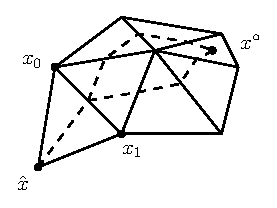
\includegraphics{nonunique.eps}
\end{center}

\begin{equation}
  x, y \in T \implies \norm{x - y}_g = \norm{x - y}_2
\end{equation}

\begin{center}
  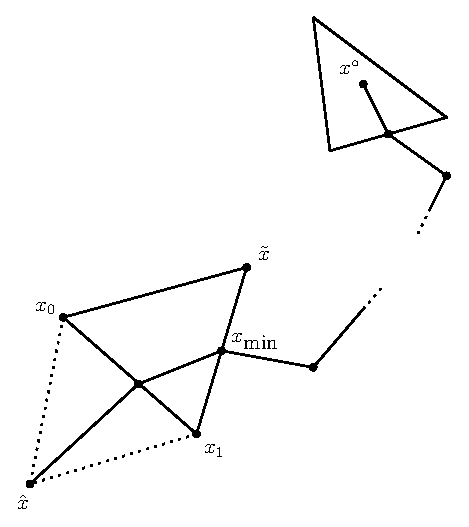
\includegraphics{recursion.eps}
\end{center}

Trying to derive some kind of recursion that will let us run the marcher...
\begin{equation}
  \norm{x_\lambda - x^\circ}_g = \min_{x \in [x_0, \tilde{x}] \cup [x_1, \tilde{x}]} \curlyb{\norm{x_\lambda - x}_2 + \norm{x - x^\circ}_g} = \norm{x_\lambda - x_{\operatorname{min}}}_2 + \norm{x_{\operatorname{\min}} - x^\circ}_g
\end{equation}

This equation will probably be useful:
\begin{equation}
  \norm{x_\lambda - x^\circ}_2^2 = (1-\lambda) \norm{x_0 - x^\circ}_2^2 + \lambda \norm{x_1 - x^\circ}_2^2 - \lambda(1-\lambda) \norm{x_1 - x_0}_2^2
\end{equation}
We may even be able to use it to obtain
$\norm{x_\lambda - x^\circ}_2^2 = d_\lambda - \lambda(1 - \lambda)
\norm{x_1 - x_0}_2^2$ recursively. This equation shows us how to
obtain $\norm{x_\lambda - x^\circ}_2^2$ by subtracting a quadratic
correction term from $d_\lambda$.

\end{document}


%%% Local Variables:
%%% mode: latex
%%% TeX-master: t
%%% End:
